\section*{3 Method}
\label{sec:method}
Figure~\ref{fig:method-overview} connects the optimization loop to the runtime that executes each candidate. We abstract this loop from the A/B/C controllers: collect parent evidence, diagnose and construct a scoped replacement, compare executions, and carry the retained program and measured feedback into the next update. We optimize a harness $H=(\lambda,G)$ around a frozen executor. Here $\lambda$ contains instructions and configuration, and $G$ specifies executable handlers, state, and dependencies. Given task distribution $D$ and normalized task score $r_H$, we minimize $\mathcal L_D(H)=1-\mathbb E_{x\sim D,\omega}[r_H(x;\omega)]$, where $\omega$ denotes execution randomness.

\begin{figure*}[!t]
\centering
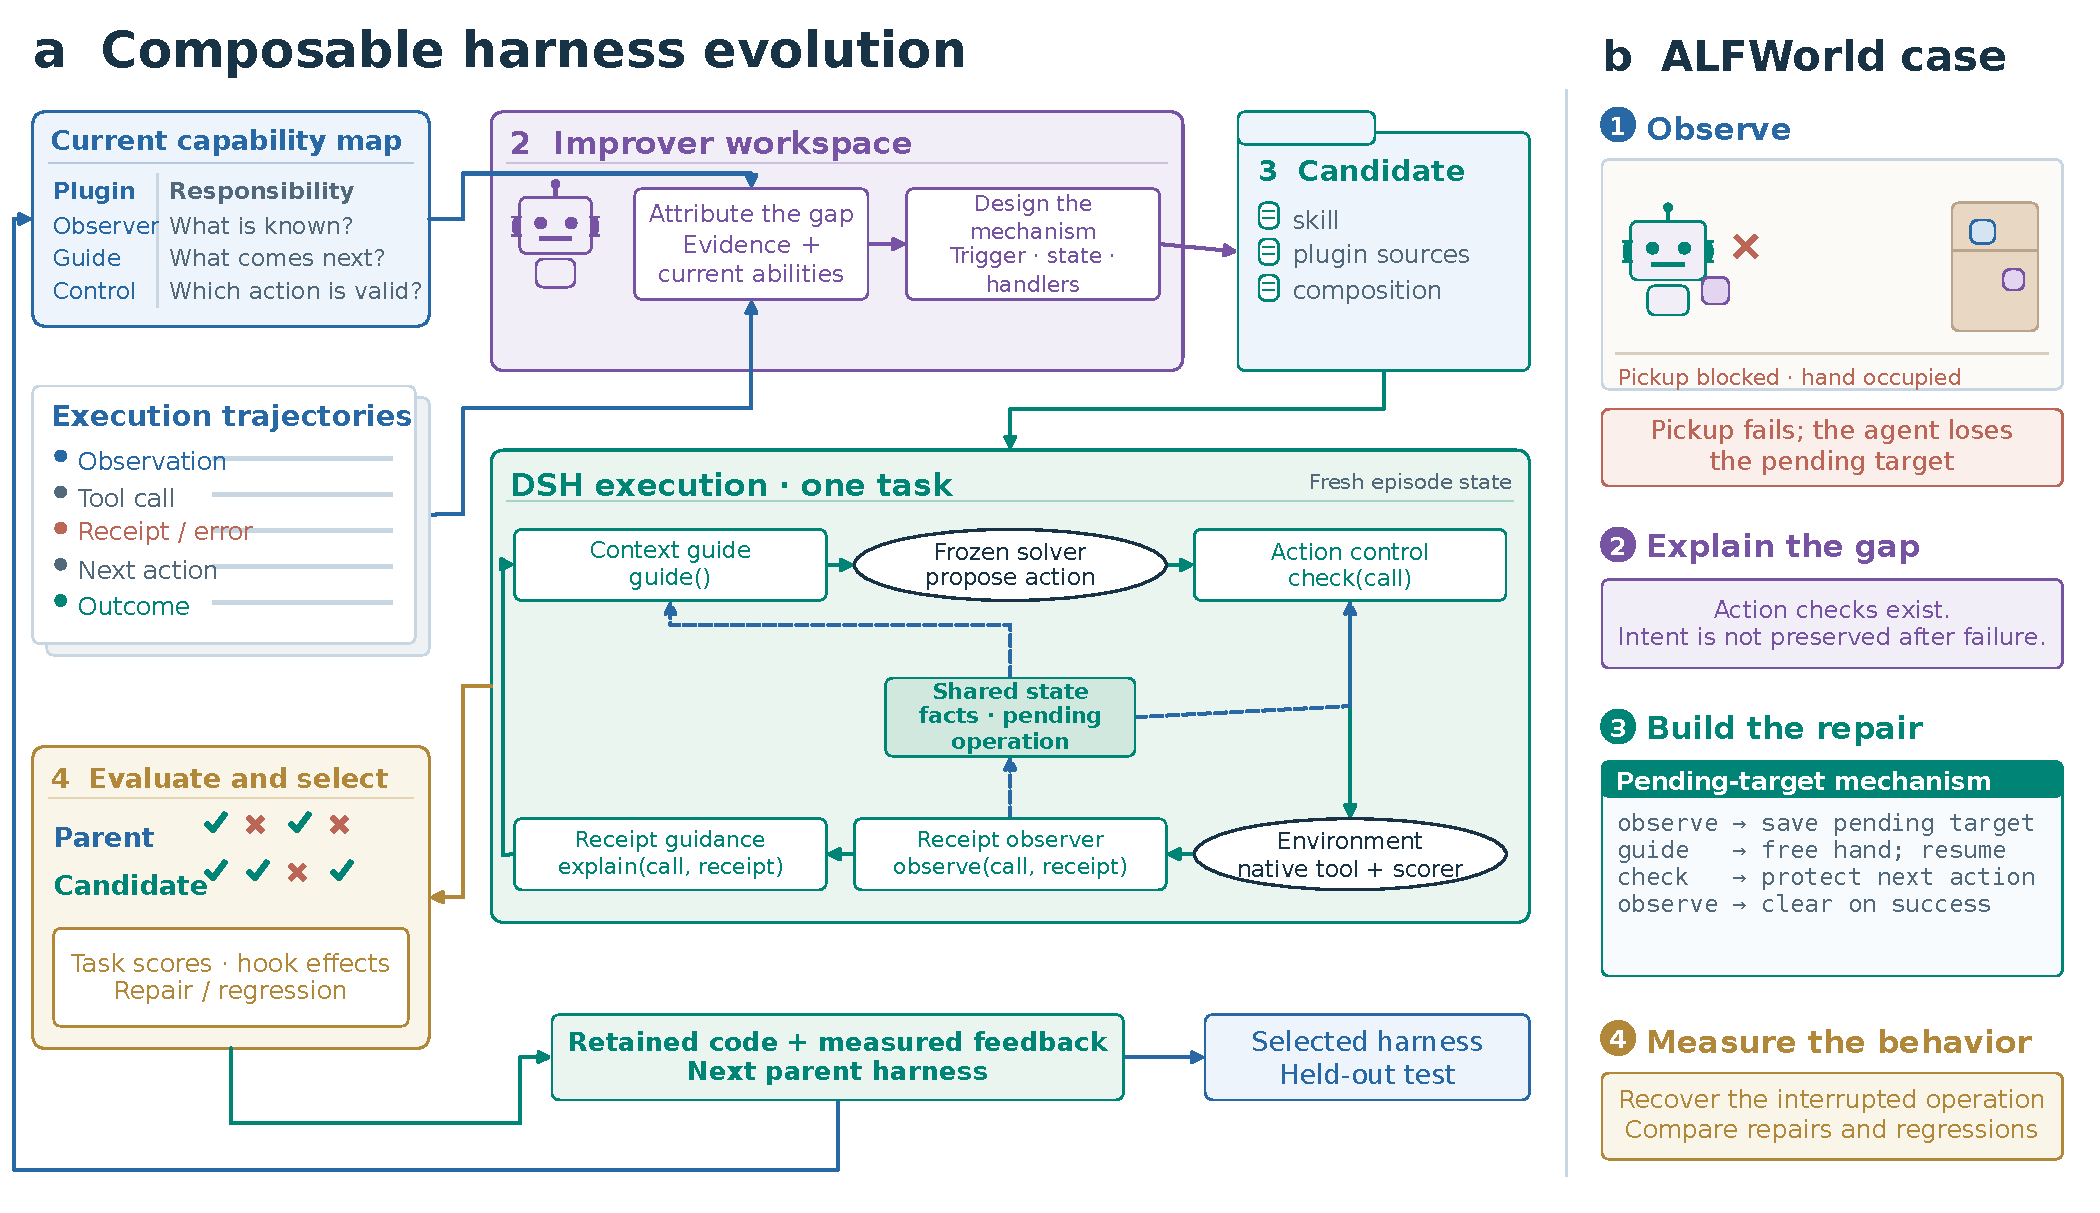
\includegraphics[width=\textwidth]{dsh-draft/figures/method-overview.pdf}
\caption{Harness evolution with composable plugins. (a) Parent capabilities and sampled trajectories enter the improver workspace, which returns a repair rationale and candidate. The candidate runs through the DSH lifecycle before paired evaluation determines the next parent and feedback. The capability map summarizes the supplied source and interfaces; attribution and design are two functions of one improver call. (b) In the illustrative ALFWorld repair, a receipt observer records a pending pickup target. Context and action handlers use that state to guide recovery.}
\label{fig:method-overview}
\end{figure*}

\subsection*{3.1 Composable Candidate Space}
DeepSeek Harness (DSH)~\citep{deepseek-harness} runs plugins at context, action, and tool-receipt hooks. Plugins can share state within an episode. This state resets for each task, while plugin code and composition persist. In the execution block of Figure~\ref{fig:method-overview}a, \texttt{guide} contributes context before the frozen solver acts, \texttt{check} can ask it to revise a tool call, and \texttt{observe} and \texttt{explain} process the returned receipt. In C, these handlers can communicate through a shared state object.

Let $\mathcal E_k(H)$ be the edits permitted under scope $k$. A revises skill text. B revises one independent component per round: skill, memory, an action check, or receipt interpretation; the remaining components are inherited. C revises skill text or jointly edits executable mechanisms and their shared state. Thus, a C candidate can connect a receipt observer, a context guide, and an action check through a common fact.

\subsection*{3.2 Observation, Attribution, and Candidate Construction}
At round $t$, execute the parent $H_t$ on batch $B_t$ and collect trajectories, task scores, and hook outputs. The controller selects successful and failed trajectories to form evidence $\mathcal T_t$. Together with the parent source and runtime interfaces $A_t$, these constitute the capabilities and execution evidence shown at the left of Figure~\ref{fig:method-overview}a. The improver also receives the previous decision $\mathcal R_t$. We express its attribution function as
\begin{equation}
g_t=\operatorname{Diagnose}_M(H_t,A_t,\mathcal T_t,\mathcal R_t).
\label{eq:direction}
\end{equation}
The diagnosis $g_t$ identifies recurring failure patterns, the evidence behind them, and the behavior to change. By relating these patterns to the current harness, the improver proposes a repair direction. This is a gradient-like direction in discrete program space~\citep{protegi,textgrad}. The proposed edit $e_t$ is the step:
\begin{align}
e_t &\sim q_M(\cdot\mid H_t,g_t,\mathcal R_t,\mathcal E_k(H_t)),\nonumber\\
H'_t&=\operatorname{Apply}(H_t,e_t).
\label{eq:proposal}
\end{align}
The improver workspace implements attribution and design in one call, returning an editable aspect, replacement content, and rationale. The controller copies the parent and installs the replacement, inheriting unedited parts. Under A this is skill text; under B it is one independent component; under C it may jointly replace skill text and a composition of named mechanisms. The proposal distribution $q_M$ thus depends on both improver capability and the permitted representation.

Figure~\ref{fig:method-overview}b illustrates this construction. A failed pickup reveals an interrupted operation whose target is no longer retained. The proposed repair connects a receipt observer that records the pending target, a guide that suggests freeing the hand and resuming, and an action check that protects the next step. An observer clears the pending state after success. C makes this producer--consumer relationship expressible within one candidate.

\subsection*{3.3 Paired Evaluation, Retention, and Feedback}
The candidate block in Figure~\ref{fig:method-overview}a contains skill text, executable sources, and their composition. Running this artifact through DSH produces the task scores and hook effects used by the evaluation block. Compare the candidate with the parent on matching tasks, trials, and seeds, using the parent outcomes collected for the current batch. For the paired evaluations $\mathcal I_t$, compute
\begin{equation}
\widehat\Delta_t=\frac{1}{|\mathcal I_t|}\sum_{i\in\mathcal I_t}
\big[r_i(H'_t)-r_i(H_t)\big].
\label{eq:paired}
\end{equation}
The controller promotes the candidate when the training objective improves, emitted hook outputs change, and the validation score does not decrease on benchmarks with a validation split. Otherwise it retains the parent. The feedback edge in Figure~\ref{fig:method-overview}a carries the latest proposal rationale, before/after scores, observed effects, repaired failures, regressions, and retention decision. The retained code becomes the next parent; a rejected edit still contributes measured feedback to the next proposal. After search, held-out evaluation measures the retained checkpoints. Appendix~A gives the general algorithm and its runtime interfaces. Appendix~B describes the A/B/C experimental setup.
